Die Entwicklung mit dem ESP Board verlief analog wie die mit dem Pretzel Board, jedoch wurden hier andere Ansätze ausprobiert.

Beispielsweise wurde der Code aufgrund seiner Kompaktheit nicht in Unterprozeduren unterteilt.
Dennoch wird in der "`setup"' Prozedur ebenfalls eine Verbindung mit dem WLAN Netzwerk hergestellt, jedoch mit der Bibliothek ESP8266WiFi.h.
In der "`loop"' Prozedur wird ebenfalls der Status des Buttons überprüft, wenn dieser gedrückt wird, wird ein tcpclient erzeugt, welcher sich mit dem Raspberry Pi verbindet, seine ID sendet und je nach Status dann entweder eine grüne oder eine rote LED leuchten lässt.
(siehe Anhang \ref{sec:CodeESP})
\begin{figure}[H]
	\centering
	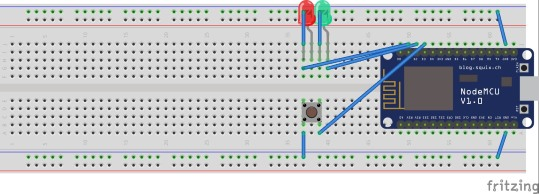
\includegraphics[scale=1.5]{ESP_Fritzing.jpg}
	\caption[ESP8266 Versuchsaufbau]{ESP8266 Versuchsaufbau,\\ Quelle: Eigener Entwurf mit Hilfe des Tools Fritzing (vgl. \cite{.fritz})}
\end{figure}